\documentclass[9pt]{beamer}

% beamerthemeFeng.sty
% style file for beamer presentation

% tikz is used to ``draw'' title page and other templates in beamer
\usepackage{tikz,etoolbox}
\usetikzlibrary{shapes,arrows}

\definecolor{UWBlack}{HTML}{000000}
\definecolor{UWWhite}{HTML}{FFFFFF}


\definecolor{UWMathPinkL1}{HTML}{FFBEEF}
\definecolor{UWMathPinkL2}{HTML}{FF63AA}
\definecolor{UWMathPinkL3}{HTML}{DF2498}
\definecolor{UWMathPinkL4}{HTML}{C60078}
\definecolor{UWGrayL1}{HTML}{DFDFDF}
\definecolor{UWGrayL2}{HTML}{A2A2A2}
\definecolor{UWGrayL3}{HTML}{787878}
\definecolor{UWGrayL4}{HTML}{000000}
\definecolor{UWGoldL1}{HTML}{FFFFAA}
\definecolor{UWGoldL2}{HTML}{FFEA3D}
\definecolor{UWGoldL3}{HTML}{FFD54F}
\definecolor{UWGoldL4}{HTML}{E4B429}

\definecolor{carrot}{HTML}{EE693F}
\definecolor{ivory}{HTML}{F1F3CE}
\definecolor{emerald}{HTML}{265C00}
\definecolor{turquise}{HTML}{5BC8AC}
\definecolor{peacockblue}{HTML}{1E656D}
\definecolor{spicy}{HTML}{B51D0A}
\definecolor{bluegreen}{HTML}{5F968E}
\definecolor{rust}{HTML}{9B4F0F}
\definecolor{burntorange}{HTML}{DE7A22}
\definecolor{sea}{HTML}{20948B}
\definecolor{lagoon}{HTML}{6AB187}


% Set colors for different components in a slide
\setbeamercolor{background canvas}{bg=UWWhite}
\setbeamercolor{author}{fg=UWGoldL3}
\setbeamercolor{institute}{fg=UWMathPinkL3}
\setbeamercolor{title}{fg=UWGrayL4}
\setbeamercolor{section in head/foot}{bg=UWBlack, fg=UWGoldL3}
\setbeamercolor{author in head/foot}{fg=UWGoldL3, bg=UWBlack}
\setbeamercolor{title in head/foot}{fg=UWBlack,bg=UWGoldL3}
\setbeamercolor{institute in head/foot}{fg=UWGoldL3, bg=UWBlack}
\setbeamercolor{navigation symbols}{fg=UWBlack}
\setbeamercolor{normal text}{fg=UWGrayL3}
\setbeamercolor{section in toc}{fg=emerald}
\setbeamercolor{subsection in toc}{fg=bluegreen}
\setbeamercolor{frametitle}{fg=UWMathPinkL2, bg=UWGrayL1}
\setbeamercolor{block title}{bg=emerald, fg=ivory}
\setbeamercolor{block body}{bg=peacockblue!20, fg=peacockblue}
\setbeamercolor{section number projected}{bg=turquise,fg=black}
\setbeamercolor{block title example}{fg=rust,
	bg= sea!40}
\setbeamercolor{block body example}{fg= burntorange,
	bg= lagoon!20}

\setbeamerfont{frametitle}{series=\bfseries} % bold frame title
\setbeamerfont{section number projected}{% bold TOC bullet
  family=\rmfamily,series=\bfseries,size=\normalsize}
  
% two common fields in conference presentations
\newcommand\jointwork[1]{\def\insertjointwork{#1}}
\newcommand\conference[1]{\def\insertconference{#1}}

% Title page style
\setbeamertemplate{title page}{
\begin{tikzpicture}[remember picture, overlay]
\fill[UWWhite]
  ([yshift=30pt]current page.west) rectangle (current page.south east);

\fill[UWBlack]
  ([yshift=30pt]current page.west) rectangle (current page.north east);

\node[anchor=east] at ([yshift=-50pt,xshift=-15pt]current page.north east)
  {
  
\includegraphics[width=0.3\linewidth]{./hselogo_fullsize_inverted.png}};

\node[anchor=north west] at ([yshift=-70pt,xshift=15pt]current page.north west) (institute)
	{
	\parbox[t]{.78\paperwidth}{
    \usebeamerfont{institute}\usebeamercolor[fg]{institute}\large\bfseries\insertinstitute}
    };
    
\node[anchor=west] at ([yshift=-45pt,xshift=15pt]current page.north west) (author)
	{
	\parbox[t]{.78\paperwidth}{
    \usebeamerfont{author}\usebeamercolor[fg]{author}\Large\bfseries \insertauthor}
    };


    
\node[anchor=north] at ([yshift=15pt]current page.center) (title)
	{
	\parbox[t]{\textwidth}{\huge\bfseries\centering
	\usebeamerfont{title}\usebeamercolor[fg]{title}\inserttitle}
	};
    
\node[anchor=north] at ([yshift=-40pt]current page.center) (jointwork)
	{
	\parbox[t]{\paperwidth}{\bfseries\centering\insertjointwork}
	};
	
\node[anchor=north] at ([yshift=40pt]current page.south) (jointwork)
	{
	\parbox[t]{\paperwidth}{\centering\insertconference}
	};
\end{tikzpicture}
}

\setbeamertemplate{headline} % add navigation to headline
{%
  \begin{beamercolorbox}{section in head/foot}
    \vskip5pt\bfseries
    \insertnavigation{\paperwidth}
    \vskip2pt
  \end{beamercolorbox}%
}


\renewcommand*{\slideentry}[6]{} % no solid circle in headline

% three-parts footline, color determined in beamer template
\setbeamertemplate{footline}
{
	\leavevmode % vertical mode is ended and horizontal mode is entered. In vertical mode, TeX stacks horizontal boxes vertically, whereas in horizontal mode, they are taken as part of the text line. 
	\begin{beamercolorbox}[wd=.333333\paperwidth,ht=2.5ex,dp=1.125ex,
      leftskip=.3cm,rightskip=.3cm plus1fil]{author in head/foot}
		\usebeamerfont{author in head/foot}\insertshortauthor
    \end{beamercolorbox}%
    \begin{beamercolorbox}[wd=.333333\paperwidth,ht=2.5ex,dp=1.125ex,
      leftskip=.3cm,rightskip=.3cm plus1fil,center]{title in head/foot}
      {\usebeamerfont{title in head/foot}\insertshorttitle}
    \end{beamercolorbox}%
    \begin{beamercolorbox}[wd=.333333\paperwidth,ht=2.5ex,dp=1.125ex,
      leftskip=.3cm,rightskip=.3cm plus1fil]{institute in head/foot}
      \hfill    {\usebeamercolor[fg]{institute in head/foot}\insertshortinstitute}    
	\end{beamercolorbox}%
}

\setbeamertemplate{navigation symbols}{\bfseries\insertframenumber/\inserttotalframenumber}

\setbeamertemplate{sections/subsections in toc}[ball]

% make the itemize bullets pixelated >
\setbeamertemplate{itemize item}{
	\tikz{
		\draw[fill=spicy,draw=none] (0, 0) rectangle(0.075, 0.075);
		\draw[fill=spicy,draw=none] (0.075, 0.075) rectangle(0.15, 0.15);
		\draw[fill=spicy,draw=none] (0, 0.15) rectangle(0.075, 0.225);
	}
}

% make the subitems also pixelated >, but a little smaller and red
\setbeamertemplate{itemize subitem}{
	\tikz{
		\draw[fill=carrot,draw=none] (0, 0) rectangle(0.05, 0.05);
		\draw[fill=carrot,draw=none] (0.05, 0.05) rectangle(0.1, 0.1);
		\draw[fill=carrot,draw=none] (0, 0.1) rectangle(0.05, 0.15);
	}
}

\AtBeginEnvironment{block}{
	\setbeamertemplate{itemize item}{
		\tikz{
			\draw[fill=spicy,draw=none] (0, 0) rectangle(0.075, 0.075);
			\draw[fill=spicy,draw=none] (0.075, 0.075) rectangle(0.15, 0.15);
			\draw[fill=spicy,draw=none] (0, 0.15) rectangle(0.075, 0.225);
		}
	}

	\setbeamertemplate{itemize subitem}{
		\tikz{
			\draw[fill=carrot,draw=none] (0, 0) rectangle(0.05, 0.05);
			\draw[fill=carrot,draw=none] (0.05, 0.05) rectangle(0.1, 0.1);
			\draw[fill=carrot,draw=none] (0, 0.1) rectangle(0.05, 0.15);
		}
	}
}

\setbeamertemplate{blocks}[rounded][shadow=false]

\setbeamercovered{invisible}

\usefonttheme[onlymath]{serif} % change the math font theme

\AtBeginEnvironment{theorem}{%
  \setbeamercolor{block title}{bg=peppercorn, fg=pearl}
  \setbeamercolor{block body}{bg=parsnip, fg=spicy}
}

\setbeamertemplate{caption}[numbered]

% set color scheme in different parts 
% please refer to beamer cheatsheet below for details
% http://www.cpt.univ-mrs.fr/~masson/latex/Beamer-appearance-cheat-sheet.pdf

\usepackage{wrapfig}

\usepackage[main=russian,english]{babel}
\usepackage[utf8]{inputenc}
\usepackage[T1,T2A]{fontenc}

\usepackage[backend=biber,style=numeric,urldate=long,maxbibnames=99,sorting=none]{biblatex}
\addbibresource{refs.bib}

\title[\textbf{PEFT}]{Parameter-Efficient Fine-Tuning} % The short title appears at the bottom of every slide, the full title is only on the title page

\author[\textbf{Алихан Зиманов}]
{Алихан Зиманов} % Your name

\institute[\textbf{ПМИ ФКН НИУ ВШЭ}] % Your institution as it will appear on the bottom of every slide, may be shorthand to save space
{Факультет компьютерных наук\\
НИУ ВШЭ % Your institution for the title page
}

\jointwork{feat. Илья Пахалко}
\conference{НИС, Москва, 2023}

%===== Uncomment the following if you wish to use references
%\usepackage[backend=bibtex,citestyle=authoryear-icomp,natbib,maxcitenames=1]{biblatex}
%\addbibresource{bibfile.bib}

% use this so appendices' page numbers do not count
\usepackage{appendixnumberbeamer}

\begin{document}

% Title page, navigation surpressed, no page number
{
\beamertemplatenavigationsymbolsempty
\begin{frame}[plain]
\titlepage
\end{frame}
}

% TOC, navigation surpressed, no page number
{
\beamertemplatenavigationsymbolsempty
\defbeamertemplate*{headline}{miniframes theme no subsection no content}
{ \begin{beamercolorbox}{section in head/foot}
    \vskip\headheight
  \end{beamercolorbox}}
\begin{frame}{Содежрание} 
\tableofcontents 
\end{frame} 
}

\addtocounter{framenumber}{-2}


\section{Введение}


\begin{frame}{Transfer Learning}

    \begin{definition}
        Применение опыта, полученного при решении одной задачи для решения новой задачи из той же области.
    \end{definition}

    \begin{example}[Классификация изображений]
        ResNet, обученный на ImageNet будет содержать в себе информацию о паттернах в картинках в целом, поэтому можно эту абстрактную информацию переиспользовать для решения других, более узких задач.
    \end{example}

    \begin{example}[Языковая модель]
        Эмбеддинги, обученные на колоссальных датасетах будут содержать в себе сложную информацию о структуре языка, поэтому их переиспользование для других задач NLP будет весьма удобным.
    \end{example}

\end{frame}


\begin{frame}{Подходы в NLP}

    \begin{block}{Pre-trained text representations (feature-based transfer)}
        Использование эбмеддингов, обученных на огромных датасетах для получения полезных признаковых описаний токенов.
    \end{block}

    \begin{block}{Fine-tuning}
        Использование уже обученной, но на другую задачу модели как инициализацию весов модели, решающей текущую задачу.
    \end{block}

    \begin{block}{Parameter-Efficient Fine-Tuning}
        Fine-tuning, обучающий как можно меньшее количество добавленных параметров или параметров исходной модели, при этом не теряющий точности решения задачи.
    \end{block}

\end{frame}

\begin{frame}{Техники обучения в NLP}

    \begin{block}{Multi-task Learning}
        Обучение модели на несколько задач одновременно. У модели имеются общие по всем задачам глубокие слои и специализированные под каждую задачу верхние слои.
    \end{block}

    \begin{block}{Continual Learning}
        Последовательное переобучение\footnote{не overfitting, а re-training} модели под каждую новую задачу.
    \end{block}

\end{frame}


\section{Adapter Tuning}

\begin{frame}{Adapter Tuning}

    Первая рассматриваемая техника PEFT это Adapter Tuning~\cite{adapter}. Хочется придумать такую технику, которая позволит решить следующие проблемы:
    
    \begin{itemize}
        \item Fine-tuning обучает все веса модели, что очень медленно и хочется обучать только малую часть весов;
        \item Multi-task learning подразумевает одновременное решение задач, что иногда бывает сложным, поэтому хочется уметь решать несколько задач, при этом не имея доступ ко всем задачам одновременно;
        \item Continual learning подразумевает дообучение имеющейся модели под новую задачу, при этом либо способность модели решать старую задачу утрачивается и сильно страдает качество, либо количество обучаемых параметров линейно возрастает с каждой следующей задачей.
    \end{itemize}

\end{frame}


\begin{frame}{Махания руками}

    Рассмотрим функцию (нейронную сеть) с параметрами $w$: $\phi_w(x)$.
    
    \begin{block}{Feature-based Transfer}
        Этот метод предлагает использовать композицию $\phi_w$ с новой функцией $\chi_v$, получая, таким образом, новую нейронную сеть $\chi_v(\phi_w(x))$. После этого обучаются только веса $v$, специфичные под текущую задачу.
    \end{block}

    \begin{block}{Fine-tuning}
        Этот метод предлагает дообучение имеющихся параметров $w$ под новую задачу, ограничивая компактность\footnote{компактная модель использует малое количество дополнительных параметров для решения новых задач} модели.
    \end{block}
    
\end{frame}


\begin{frame}{Махания руками 2.0}
    
    \begin{block}{Adapter tuning}
        Этот метод предлагает ввести новую функцию $\psi_{w, v}(x)$, где $w$ это в точности те же параметры, что и в $\phi_w$. Новые параметры $v$ инициализируются так, чтобы новая функция повторяла исходную: $\psi_{w, v_0}(x) \approx \phi_w(x)$. Во время обучения обновляются только веса $v$, а $w$ остаются неизменными. В идеале мы хотим строить функции $\psi$ такие, что $|v| \ll |w|$, чтобы размер модели практически не возрастал при добавлении новых параметров.
    \end{block}

    \begin{block}{Как это делать?}
        Для решения каждой новой задачи между слоями исходной модели будем добавлять новые, так называемые, adapter слои. В процессе обучения обновляться будут только веса этих добавленных слоев.
    \end{block}

\end{frame}


\begin{frame}{Adapter tuning для трансформеров}

    \begin{columns}
        \column{0.45\textwidth} \begin{figure}
            \caption{Слева блок трансформера, справа слой адаптера}
            \label{adapter:block}
            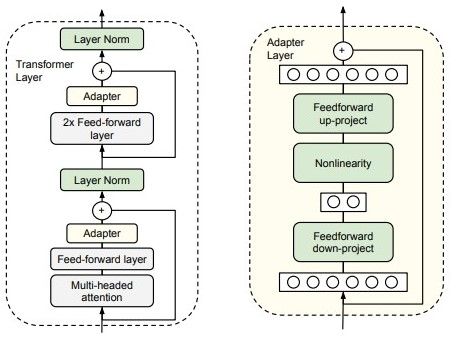
\includegraphics[scale=0.5]{images/adapter_1.jpg}
        \end{figure}
        \column{0.55\textwidth} \begin{block}{Transformer}
            В трансформере есть два главных типа слоёв: \textit{attention} слой и \textit{feedforward} слой. Слой \textit{adapter} добавляется сразу после каждой пары указанных слоев, но перед слоем нормализации и перед \textit{skip connection} слоем.
        \end{block} \begin{block}{Adapter}
            Слой адаптера по смыслу сначала проецирует $d$-мерные вектора признаков в меньшее $m$-мерное пространство, применяют нелинейность и проецируют вектора обратно в $d$-мерное пространство, добавив skip connection.
        \end{block}
    \end{columns}

\end{frame}


\begin{frame}{Махания руками 3.0}

    \begin{block}{Количество параметров}
        Заметим, что количество обучаемых параметров в одном adapter слое будет $2 m d + d + m$. Если брать $m \ll d$, мы можем легко ограничить количество добавляемых параметров для решения новой задачи. На практике можно добиться добавления всего $0.5 - 8\%$ параметров от исходной модели.
    \end{block}

    \begin{block}{Инициализация}
        Если инициализировать веса adapter слоя околонулевыми числами, то skip connection слой позволит новой модели имитировать исходную модель.
    \end{block}

    \begin{block}{Удобно?}
        Да\footnote{потому что новые задачи не портят качество на старых задачах в силу неизменения старых весов и количество новых параметров очень мало}.
    \end{block}
    
\end{frame}


\begin{frame}{Эксперименты}
    
    \begin{block}{Результаты}
        На GLUE бенчмарке adapter tuning позволяет достичь результата в диапазоне $0.4\%$ от fine-tuning всех параметров модели BERT, при этом adapter tuning добавляет и обучает всего $3\%$ от общего количества параметров модели.
    \end{block}

    \begin{figure}
        \begin{center}
            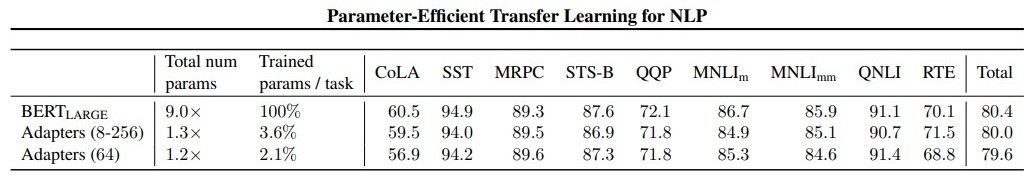
\includegraphics[scale=0.45]{images/adapter_2.jpg}
        \end{center}
    \end{figure}

\end{frame}


\section{Prefix-Tuning}

\begin{frame}{Prefix-Tuning}

    \begin{block}{Prefix-tuning}
        Вторая рассматриваемая техника PEFT это Prefix Tuning~\cite{prefix}. Эта техника пытается решить те же проблемы, что и adapter tuning, а именно обучаться на новые задачи не теряя способности решать старые, а также обучение минимального количества весов модели\footnote{оказывается у этого есть название --- lightweight fine-tunning}, чтобы для новых задач не требовалось хранить полные копии исходной модели.
    \end{block}

    \begin{block}{Задачи}
        Авторы статьи предлагают применить эту технику для задач типа table-to-text и summarization.

        \begin{itemize}
            \item Table-to-text --- генерация текстового описания объекта по структурированному табличному описанию. Например, из табличного представления $(\text{name}: \text{'Starbucks'}, \text{type}: \text{'coffee shop'})$ хотим получить текстовое описание: 'Starbucks serves coffee'.
            \item Summarization --- генерация краткого текстового описания более длинного исходного текста.
        \end{itemize}

    \end{block}

\end{frame}


\begin{frame}{Махания руками}

    \begin{block}{Контекст}
        В языковых моделях для генерации текста используются векторы контекста\footnote{вспоминаем рекуррентные нейронные сети}, призванные помогать модели понимать, что ей следует предсказывать дальше.
    \end{block}

    \begin{block}<2->{Гениальная идея}
        Можно ли придумать такой контекст в виде префикса, дописываемого перед каждыми входными данными, который будет указывать модели не просто генерируемый результат, а саму задачу, которая модель должна решать?

        \begin{solution}<3->
            Да!
        \end{solution}
    \end{block}

\end{frame}


\begin{frame}{Красивая картинка}
    \begin{figure}
        \caption{Добавление контекста в префикс входных данных и сравнение с полным fine-tuning}
        \begin{center}
            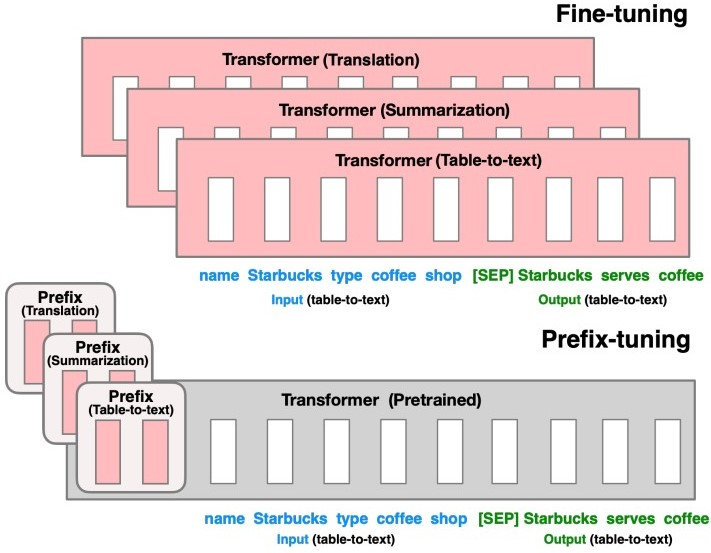
\includegraphics[scale=0.5]{images/prefix_1.jpg}
        \end{center}
    \end{figure}
\end{frame}


\begin{frame}{Эксперименты}
    
    \begin{block}{Датасеты}
        Для table-to-text задачи использовались датасеты E2E, WebNLG и DART, а для summarization использовался XSUM.
    \end{block}
    
    \begin{block}{Архитектуры}
        Для table-to-text использовались $\text{GPT-2}_{\text{MEDIUM}}$ и $\text{GPT-2}_{\text{LARGE}}$. Для summarization использовался $\text{BART}_{\text{LARGE}}$.
    \end{block}

\end{frame}

\begin{frame}{Результаты}

    \begin{block}{Table-to-text}
        Как видно по таблице~\ref{prefix:table-to-text}, prefix-tuning обходит другие бейзлайны\footnote{Adapter и FT-TOP2} добавляя всего лишь $0.1\%$ параметров и имеет качество, сравнимое с полным fine-tuning на всех трех датасетах. Если уменьшить количество параметров для метода adapter до тех же $0.1\%$, его качество станет сильно хуже prefix-tuning.
    \end{block}

    \begin{block}{Summarization}
        Судя по таблице~\ref{prefix:summarization}, prefix-tuning уже уступает полному fine-tuning в силу более сложного датасета.
    \end{block}

\end{frame}

\begin{frame}{Таблица}

    \begin{figure}
        \label{prefix:table-to-text}
        \caption{Table-to-text}
        \begin{center}
            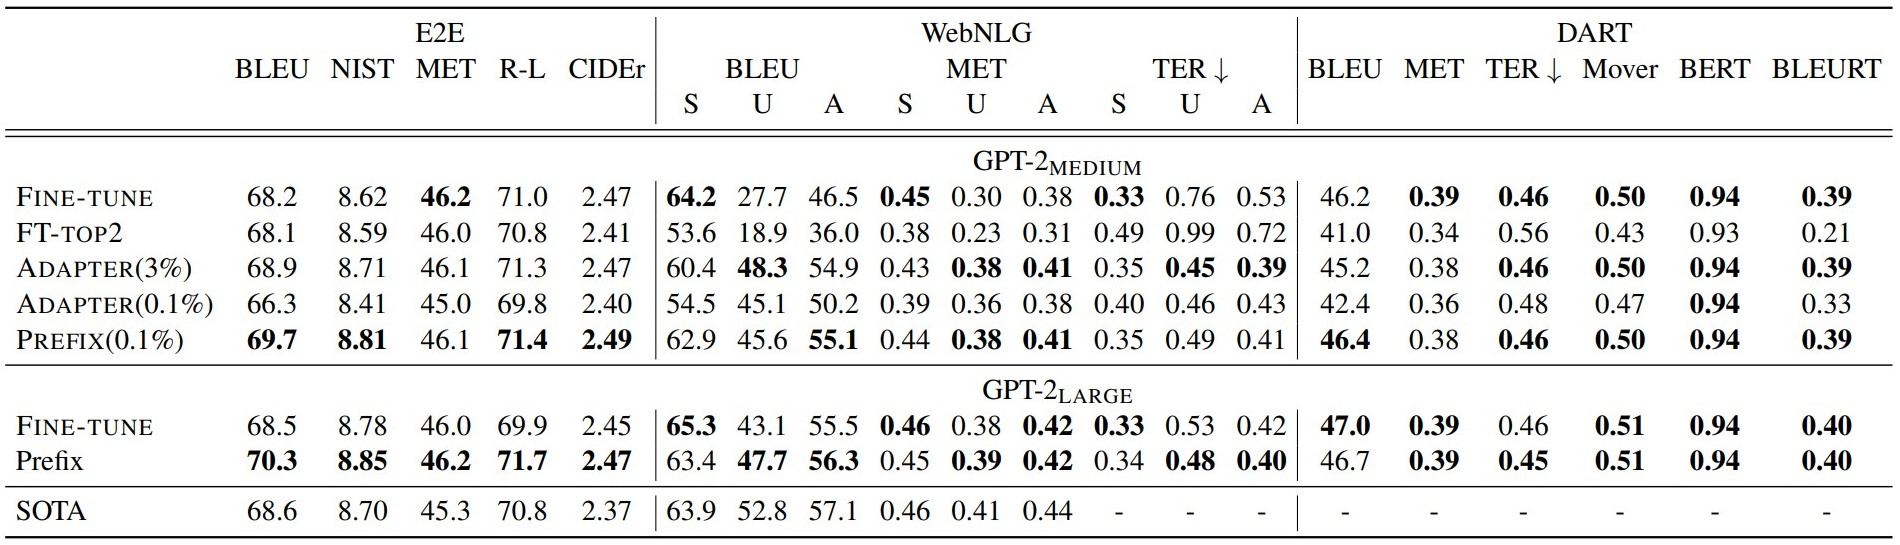
\includegraphics[scale=0.27]{images/prefix_2.jpg}
        \end{center}
    \end{figure}

    \begin{figure}
        \label{prefix:summarization}
        \caption{Summarization}
        \begin{center}
            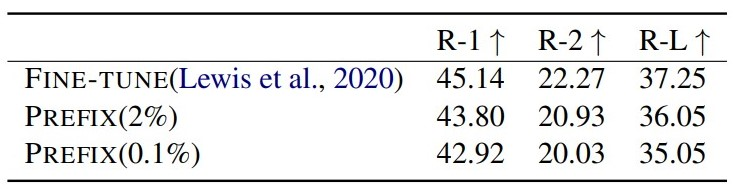
\includegraphics[scale=0.3]{images/prefix_3.jpg}
        \end{center}
    \end{figure}

\end{frame}

\section{LoRA}

\begin{frame}{LoRA}
    Последняя рассматриваемая техника PEFT это LoRA~\cite{lora}, то есть Low-Rank Adaptation of Large Language Models.
\end{frame}


\begin{frame}[allowframebreaks]
    \frametitle{Список литературы}
    \printbibliography
\end{frame}


\end{document}